

\section{The LHCb Experiment}
%\cite{LHCb}
The LHCb detector is designed specifically to study $CP$ violation and rare decays of $b$-hadrons and $c$-hadrons building on work done a the B factories and the Tevatron.
At the high energies the LHC operates at $b\bar{b}$ pairs are produced together at low polar angles in either the forwards or backwards cone along the 
beam direction. The detector is designed as a single-arm spectrometer to take advantage of this behaviour.


A cross-section of the detector layout is shown in Fig.~\ref{LHCb}. 

\begin{figure}[htb]
\centering
  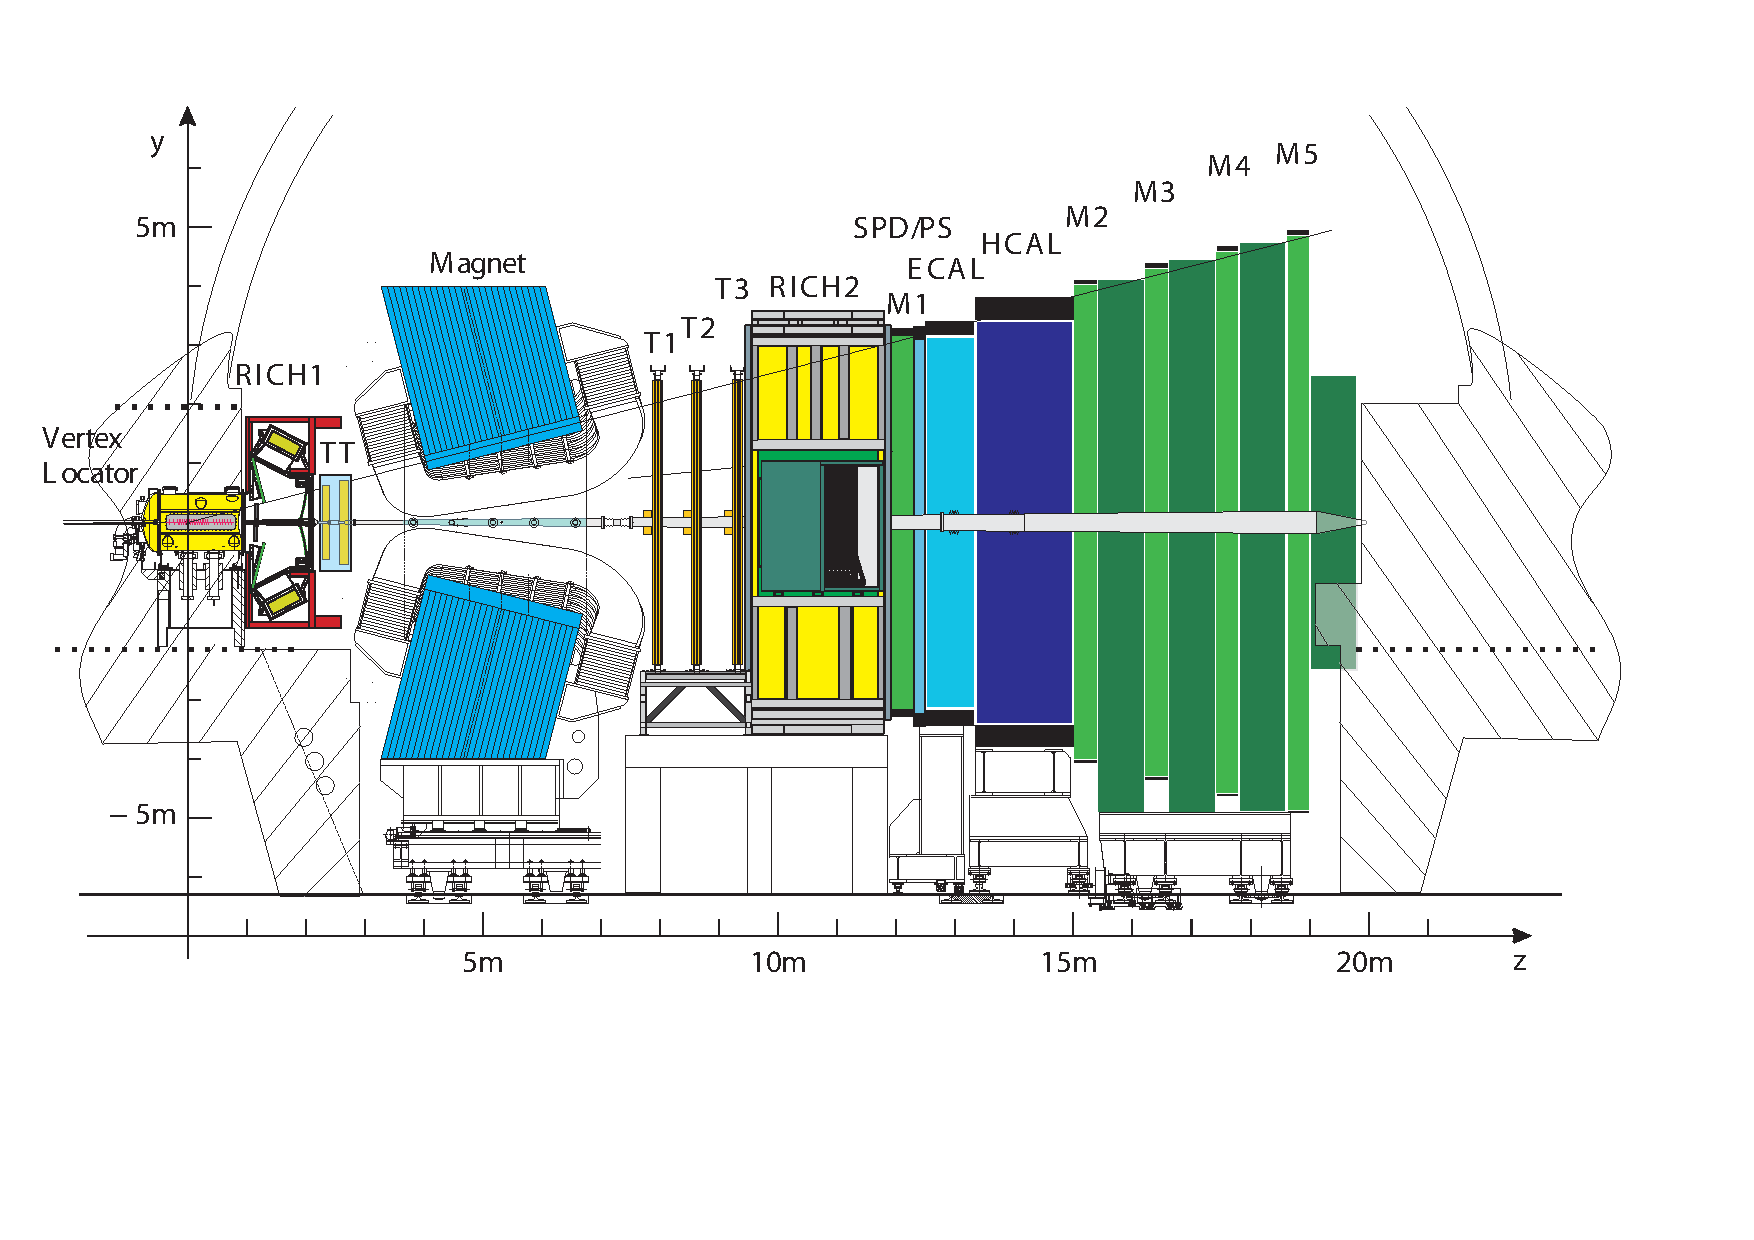
\includegraphics[width = 0.85 \linewidth]{lhcb.pdf}
  \caption{Cross-section of the LHCb detector the the $z$-axis is along the beam pipe and the $y$-axis is the vertical direction \cite{LHCb}.}
  \label{LHCb}
\end{figure}

The LHCb detector is composed of sub-detectors with different design purposes. The vertex locator (VELO) 
and the tracking stations (TT, T1, T2 and T3) are key for tracking charged particles travelling through
the detector. The RICH detectors, calorimeters (ECAL, HCAL, PS and SPD) and the muon stations (M1-5) 
are necessary for particle identification. The dipole magnet in the detector is used alongside the tracking stations in order to measure particle charge and momentum.


The VELO is the tracking detector closest to the interaction point. It is designed to locate primary and secondary decay vertices. Secondary vertices occur within the VELO
due to the short lifetime of $b$-hadrons, whereas primary vertices do not occur in the VELO but tracks in the VELO are extrapolated backwards to determine the vertex location.
The VELO is a silicon micro-strip detector which give good resolution of tracks and decay vertices. 




The T1-3 tracking station consist of the Inner Tracker (IT) and the Outer Tracker (OT). The IT is a silicon micro-strip detector and makes up the inner sections of the stations closest to the beam pipe.
The OT is a straw-tube drift-chamber and covers the outer sections of the T1-3 stations. Silicon micro-strip detectors are needed in the IT due to high particle occupancy however the particle flux is lower at large polar angles from the beam pipe allowing straw tubes to be used
in the OT as the occupancy is lower. The Tracker Turicensis (TT) is also a silicon micro-strip detector upstream of IT and OT, it spans the full acceptance of the LHCb detector. The TT, IT and OT work together with the dipole magnet to measure charge and momentum of particles travelling through the detector. Obtaining good momentum resolution is vital because the momentum resolution 
directly affect the invariant mass resolution of reconstructed particles. 

Distinguishing between $e$, $\mu$, p, K, $\pi$ and photons is important for accurately reconstructing particle decays. Each sub-detector related to particle identification is specialised for
 different particles. The sub-detectors for particle identification are the two RICH detectors, the Preshower detector (PS), Scintillating Pad Detector (SPD), the electromagnetic calorimeter (ECAL), the hadronic calorimeter 
(HCAL) and the muon tracking stations (M1-5). 

The particle identification detectors closest to the interaction point are the RICH~1 and RICH~2. These detectors are ring imaging $\check{\text{C}}$erenkov detectors, designed to separate charged pions and kaons
 which are produced in large number from $b$-hadron decays.  In LHCb, high momentum particles are produced at small polar angles and lower momentum particles at larger polar angles, therefore two RICH 
detectors are needed to cover the full momentum and acceptance range. The RICH 1 is composed of an areogel and $C_{4}F_{10}$ gas radiator, it is sensitive to particles with momentum between  1 and 60 G$e$V/$c$. 
The RICH 2 is a $CF_{4}$ gas radiator and is sensitive to particles with momentum between 15 and 100 G$e$V/$c$. 


The SPD distinguishes charged and neutral particles such as photons and electrons which leave the same signals in the ECAL. The PS detector distinguishes electrons and 
charged pions by utilising their different interaction lengths in matter. 


Downstream of the SPD and the PS is the ECAL, a lead-scintillator sampling detector. Electrons and photons interact within the lead producing electromagnetic showers, the scintillator 
absorbs photons produced by the showers and emits photons at different wavelengths so that photomultiplier tubes detect them. The energy of an incident particle is measured from the energy of the shower which is proportional to the light produced in the shower. Showers produced by photons can be distinguished from those produced by electrons because photons leave no hits 
in the tracking detectors or the SPD. Hadrons will pass though the ECAL to be detected by the HCAL. The HCAL is composed of lead and scintillator tiles and measure the energy 
hadronic showers produced inside it. The HCAL works in the same way as the ECAL however the lead absorber is more suited to producing hadronic showers rather than electromagnetic ones.

Muon identification is key for the analysis of several important CP violating decays and rare decays, including $B_{s} \to \mu^{+} \mu^{-}$. The ECAL and the HCAL absorb most particles produced in collisions. 
However, the high penetration power of muons allows then to pass through the ECAL and HCAL therefore the muon stations can be the in furthest part of the detector.  The muon stations are multi-wire proportional chambers except the inner part of the M1 station which is 
a gas electron multiplier due to the high particle occupancy. 


Muon identification is not only important for offline analysis but, together with information from the ECAL and HCAL, the muon system triggers events which are saved for offline analysis. 
The LHCb has been designed to operate at a lower instantaneous luminosity than the running of the LHC, the trigger takes the 10 MHz of data visible in the LHCb and reduces it to 5 kHz which can 
be stored offline. There are two levels to the trigger the Level 0 (L0) and the High Level Trigger (HLT). The L0 operates at the same time as the bunch crossings and reduced the rate to 1 MHz
by using transverse momentum information from the ECAL, HCAL and the muon stations. The HLT further reduces the rate to 5 kHz, running asynchronously with the bunch crossings on a processor farm. The HLT
takes events that have been triggered by the L0 and confirms them by reconstructing the events more fully using information from the VELO and other tracking stations. Once the data has been stored there are further offline selections
which aim to further reduce the background and enhance the signal for particular decays.  The trigger is optimised so when it is combined with the offline selection it can give the best signal and best background rejection. Since the LHCb studies many different decays there are various different
triggers that are used for different analyses. 




%Things to note and change:
%The IT and OT it's not really about resolution but about occupancy. There can only be one event hit per strip so that the reading makes sense and isn't useless. If a straw tube, which is 
%v long, gets more that 1 hit the readout is useless, since there are more particles in at small polar angles we need more/smaller detectors so that the occupancy of each detector is smaller.
%Can't have SMD over all the detector because it is too expensive.

%The trigger number are probably wrong now, it was bten 4 and 6 kHz in 2012. Also would be good to add in more details about how the trigger works. 

%Add in that the PS-HCAL get rid of all/many the other particles which are not muons therefore allowing the M2-5 to detect what is left which are muons.

